\documentclass{beamer} 
\usepackage{amsmath,amsthm}
\usepackage{graphicx,microtype,parskip}
\usepackage{caption,subcaption,multirow}
\usepackage{attrib}
\usepackage{array}

\frenchspacing

\usetheme{default}
\usecolortheme{whale}

\setbeamertemplate{navigation symbols}{}

\setbeamercolor{title}{fg=blue,bg=white}

\setbeamercolor{block title}{fg=white,bg=gray}
\setbeamercolor{block body}{fg=black,bg=lightgray}

\setbeamercolor{block title alerted}{fg=white,bg=darkgray}
\setbeamercolor{block body alerted}{fg=black,bg=lightgray}


\title{Regression}
\date{}

\begin{document}


\begin{frame}
  \maketitle
\end{frame}


\begin{frame}
  \frametitle{Today's goals}

  \begin{itemize}
    \item introduce linear regression models
    \item learn to interpret the parameters of a regression model
    \item Identify the assumptions of linear regression
    \item Share some useful protips
    \item introduce logistic regression (if we have time)
  \end{itemize}
\end{frame}


\begin{frame}
  \frametitle{Definition linear regression}

  \begin{Large}
    \dots a method that summarizes how the average values of a numerical \textit{outcome} variable vary over subpopulations defined by linear functions of \textit{predictors}. \dots Regression can be used to predict an outcome given a lienar function of these predictors, and regression coefficients can be thought of as comparisons across predicted values or as comparisons among averages in the data.
  \end{Large}

  \attrib{\footnotesize{Gelman and Hill, 2007, p.31}}
\end{frame}


\begin{frame}
  \frametitle{What is linear regression?}

  \begin{itemize}
    \item simple statistical model
    \item model of mean and variance of normally (Gaussian) distributed variance
    \item mean as \textit{additive} combination of \textit{weighted} variables
    \item constant variance
  \end{itemize}
\end{frame}


\begin{frame}
  \frametitle{Linear models}

  \begin{itemize}
    \item models of normally distributed data
      \begin{itemize}
        \item t-test, single regression, multiple regression, ANOVA, ANCOVA, MANOVA, MANCOVA
        \item all just special cases of linear regression
      \end{itemize}
    \item focus on the strategy, not the magic words
  \end{itemize}
\end{frame}


\begin{frame}
  \frametitle{One predictor}

  \(y\) is a continuous variable defined for \(-\infty\) to \(\infty\) (e.g. test score)

  \(x\) is a vector of 0s and 1s (e.g. completed high school)

  \begin{align*}
    y &= \alpha + \beta x + \epsilon \\
    \epsilon &\sim \text{Normal}(0, \sigma)
  \end{align*}
\end{frame}


\begin{frame}
  \frametitle{Parts of this model}

  \begin{align*}
    y &= \alpha + \beta x + \epsilon \\
    \epsilon &\sim \text{Normal}(0, \sigma)
  \end{align*}

  \begin{columns}
    \begin{column}{0.5\textwidth}
      \begin{itemize}
        \item \(\alpha\)
          \begin{itemize}
            \item ``the intercept''
            \item expected value of \(y\) when all \(x\) are 0
          \end{itemize}
        \item \(\beta\)
          \begin{itemize}
            \item regression coefficient 
            \item expected change in \(y\) per unit change in \(x\)
          \end{itemize}
      \end{itemize}
    \end{column}
    \begin{column}{0.5\textwidth}
      \begin{itemize}
        \item \(\epsilon\)
          \begin{itemize}
            \item ``error'' term
            \item describes the residuals -- the dispersion around the linear element
          \end{itemize}
        \item \(\sigma\)
          \begin{itemize}
            \item standard deviation of dispersion around linear element
          \end{itemize}
      \end{itemize}
    \end{column}
  \end{columns}
\end{frame}

\begin{frame}
  \frametitle{Another way to write out linear model}
  \begin{align*}
    y &= \alpha + \beta x + \epsilon \\
    \epsilon &\sim \text{Normal}(0, \sigma)
  \end{align*}

  \begin{center}
    is the same as
  \end{center}

  \begin{align*}
    y &\sim \text{Normal}(\alpha + \beta x, \sigma)
  \end{align*}
\end{frame}

\begin{frame}
  \frametitle{Regression coefficients}

  \begin{Large}
    The expected difference in \(y\) between two units that differ by 1 in a single predictor.
  \end{Large}
\end{frame}


\begin{frame}
  \frametitle{One predictor}
  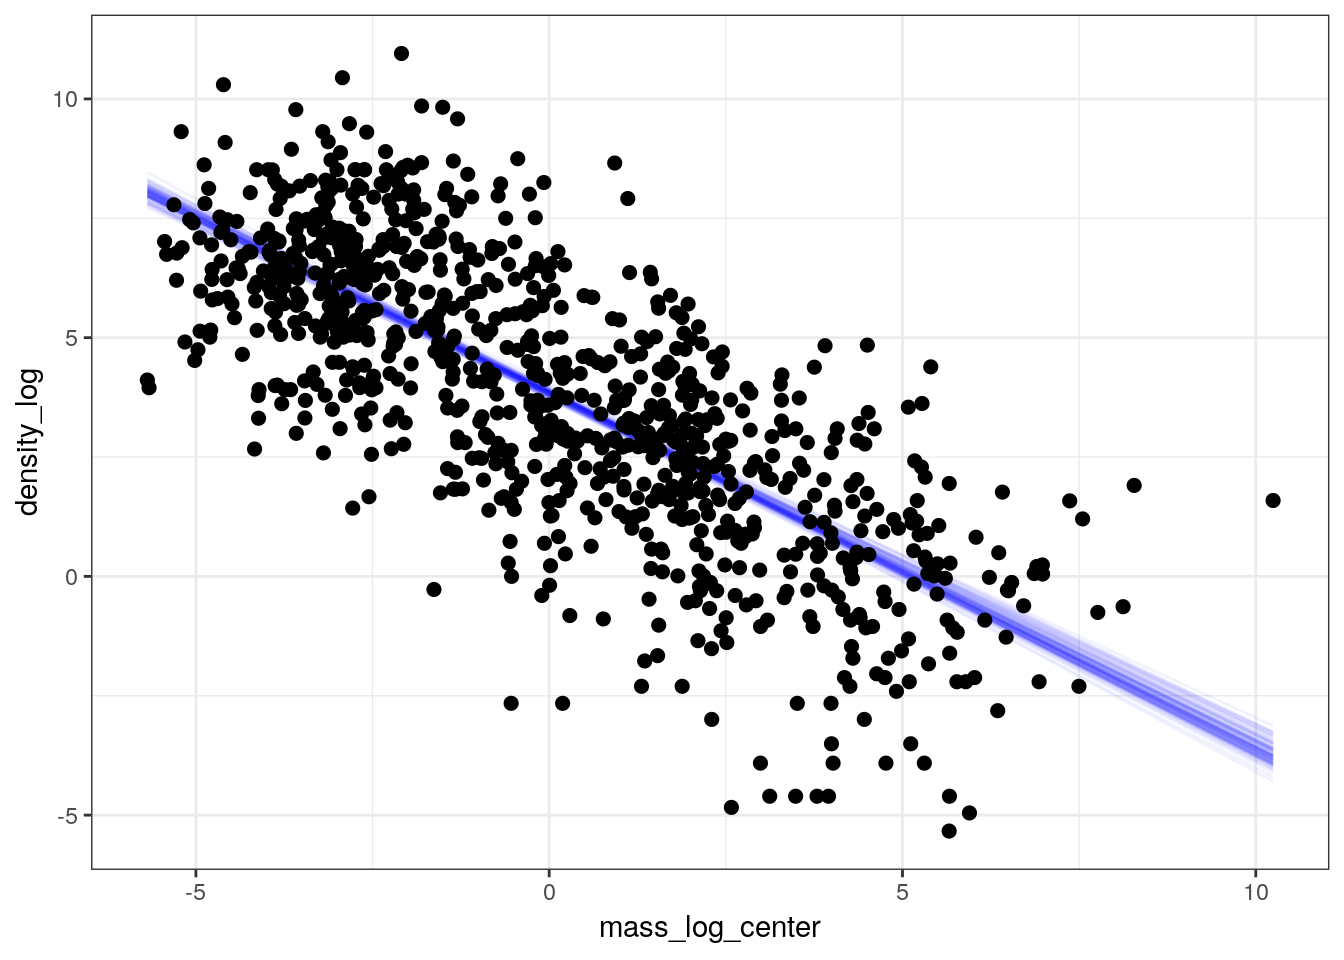
\includegraphics[width=\textwidth,height=0.8\textheight,keepaspectratio=true]{predictor_fitted-1}
\end{frame}


\begin{frame}
  \frametitle{One \textit{binary} predictor}

  For a binary predictor, the regression coefficient is the difference between the averages of the two groups.

  \attrib{\footnotesize{Gelman and Hill, 2007, p.31}}
\end{frame}

\begin{frame}
  \frametitle{One \textit{binary} predictor}
  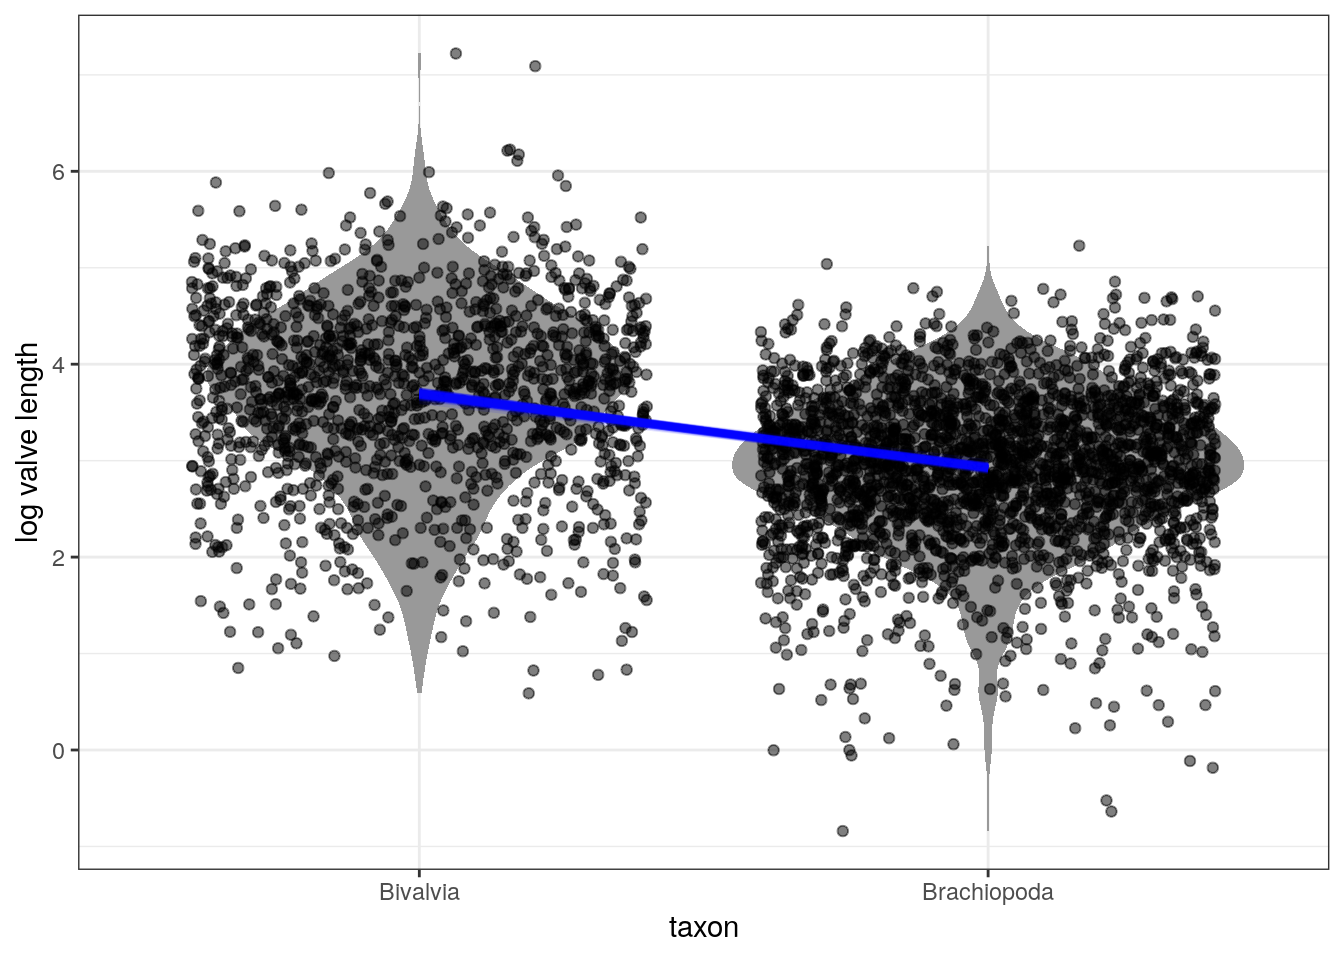
\includegraphics[width=\textwidth,height=0.8\textheight,keepaspectratio=true]{vis_linear_predictor_uncertainty-1}
\end{frame}


\begin{frame}
  \frametitle{Multiple predictors}

  \begin{Large}
    Typical advice is to interpret each coefficient ``with all the other predictors held constant.''
  \end{Large}
  
  \attrib{\footnotesize{Gelman and Hill, 2007, p.31}}
\end{frame}

\begin{frame}
  \frametitle{Multiple predictors\dots what?}
  
  \begin{align*}
    y &\sim \text{Normal}(\alpha + \beta_{1} x_{1} + \beta_{2} x_{2}, \sigma)
  \end{align*}

  \(\beta_{1}\) only describes change in y based on \(x_1\). changing \(x_{2}\) is assumed indendent.
\end{frame}

\begin{frame}
  \frametitle{Multiple predictor}
  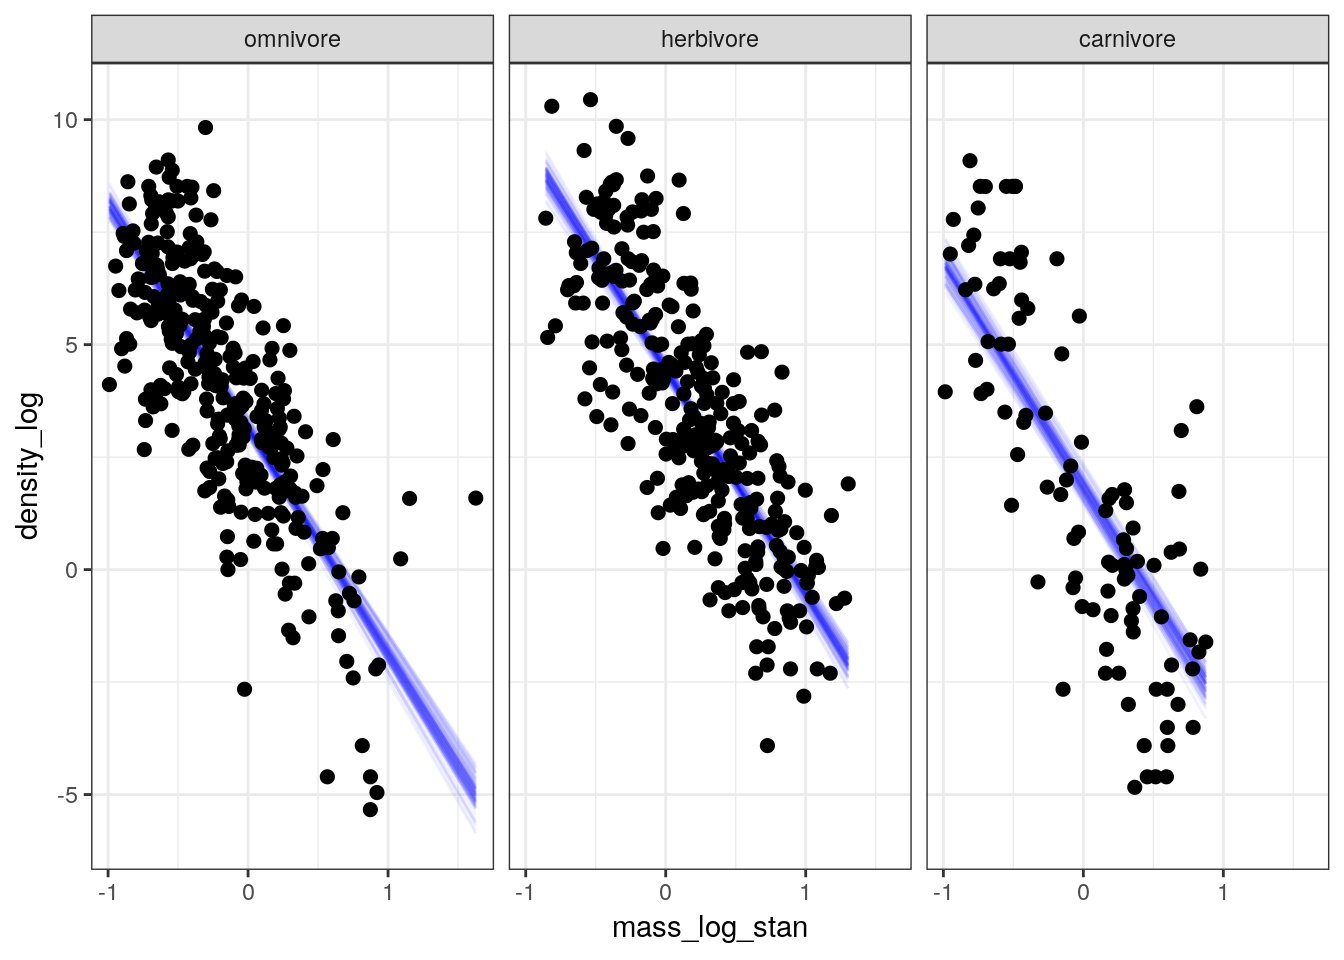
\includegraphics[width=\textwidth,height=0.8\textheight,keepaspectratio=true]{multi_fitted-1}
\end{frame}

\begin{frame}
  \frametitle{Vector-matrix notation}

  \begin{align*}
   \alpha + \beta_{1} x_{1} + \beta_{2} x_{2} &= \alpha + X\beta
  \end{align*}

  \begin{center}
    or, if first column of X is all 1s
  \end{center}

  \begin{align*}
    \beta_{0} + \beta_{1} x_{1} + \beta_{2} x_{2} &= X\beta
  \end{align*}
\end{frame}


\begin{frame}
  \frametitle{Assumptions}
  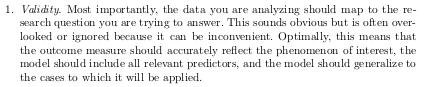
\includegraphics[width=\textwidth,height=0.5\textheight,keepaspectratio=true]{assumption_1}

  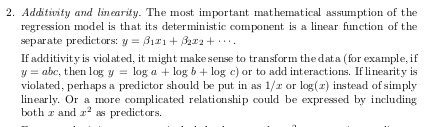
\includegraphics[width=\textwidth,height=0.5\textheight,keepaspectratio=true]{assumption_2}
\end{frame}


\begin{frame}
  \frametitle{Assumptions}
  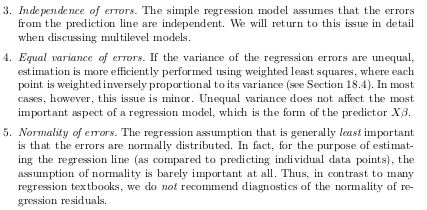
\includegraphics[width=\textwidth,height=0.8\textheight,keepaspectratio=true]{assumption_3}
\end{frame}


\begin{frame}
  \frametitle{Advice}
  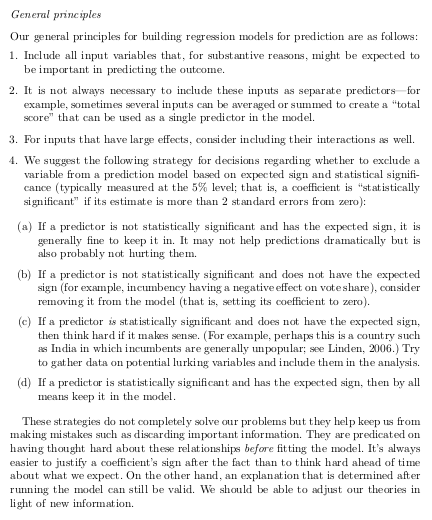
\includegraphics[width=\textwidth,height=0.8\textheight,keepaspectratio=true]{advice}
\end{frame}


%\begin{frame}
%  \frametitle{PROTIPS}
%
%  \begin{itemize}
%    \item mean-center and unit-scale your data -- helps interpreting coefficients
%      \begin{itemize}
%        \item \(x_{rescale} = \frac{x - \bar{x}}{\text{sd}(x)}\)
%      \end{itemize}
%    \item log contiunous predictors that are bound to be \(>\) 0
%    \item if \(\sigma\) is the residual standard deviation, then \(R^2 = 1 - \frac{\sigma}{\text{sd}(y)}\) 
%  \end{itemize}
%\end{frame}



\begin{frame}
  \frametitle{Logistic regression}

  \begin{center}
    The standard way to model binary outomes.
  \end{center}

  \begin{align*}
    \text{Pr}(y_{i} = 1) &= \text{logit}^{-1}(X_{i}\beta)
  \end{align*}
\end{frame}

\begin{frame}
  \frametitle{Logit, or log-odds, function}

  \[
    \text{logit}(p) = \text{log} \frac{p}{1 - p}
  \]

  \begin{center}
    maps continuous space from \(-\infty\) to \(\infty\) to (0, 1).
  \end{center}

\end{frame}

\begin{frame}
  \frametitle{Logit, or log-odds, function}

  \begin{columns}
    \begin{column}{0.5\textwidth}
      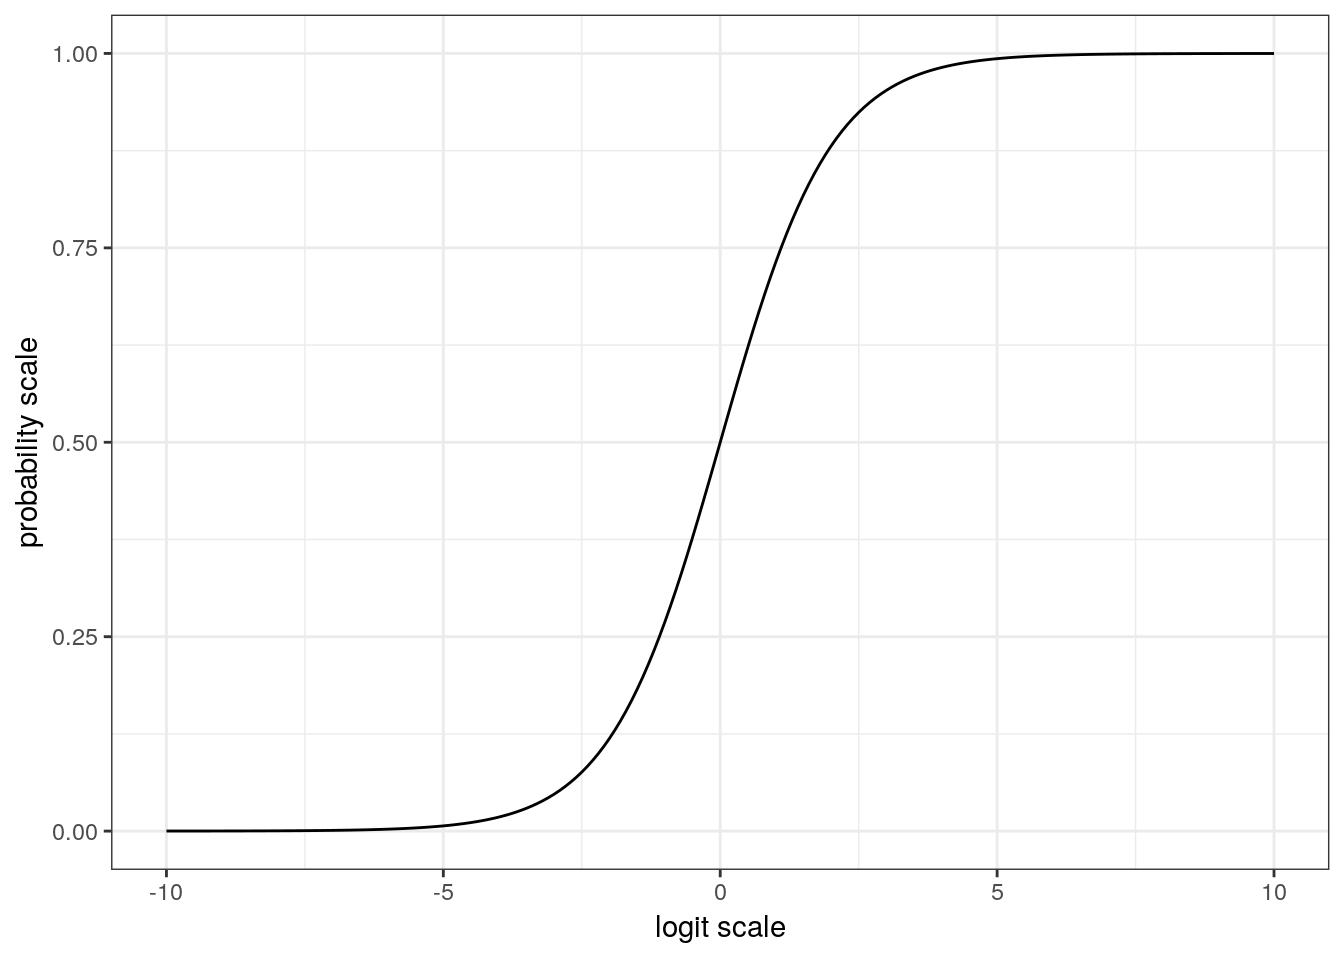
\includegraphics[width=\textwidth,height=0.8\textheight,keepaspectratio=true]{logisitic-demo-1}
    \end{column}
    \begin{column}{0.5\textwidth}
      When \(x\) has a magnitude of 3 , \(y\) is either close to its maxima or minima. The approximate slope of the logistic function for \(x\) between -3 and 3 is much larger than the slope of the logistic function for values with a magnitude of 3+. Any change on the logit scale is compressed at the ends of the probability scale.
    \end{column}
  \end{columns}
\end{frame}

\begin{frame}
  \frametitle{Alternative notation}

  \begin{align*}
    \text{Pr}(y_{i} = 1) &= \text{logit}^{-1}(X_{i}\beta)
  \end{align*}

  \begin{center}
    is the same as
  \end{center}

  \begin{align*}
    y_{i} &\sim \text{Bernoulli}(\theta_{i}) \\
    \theta_{i} &= \text{logit}^{-1} (X_{i} \beta)
  \end{align*}
\end{frame}

\begin{frame}
  \frametitle{Interpreting logistic regression coefs}

  The definition of a regression coefficient is that it describes the expected change in the response per unit change in its predictor. However, the logit (or inverse logit) function introduced into our model creates a nonlinearity which complicates the simplicity of this interpretation. 

  \begin{align*}
    y &\sim \text{Bernoulli}(\theta) \\
    \theta &= \text{logit}^{-1}(-1 + -0.5 x) \\
  \end{align*}

\end{frame}

\begin{frame}
  \frametitle{Interpreting logistic regression coefs: intercept}

  The intercept of a logistic can only be interpreted assuming zero values for all the other predictors. This point is where on the probability axis the logistic function crosses $x = 0$. 
  
  With mean-centered data, the central point describes the baseline probability of the result being a 1. 
\end{frame}

\begin{frame}
  \frametitle{Interpreting logistic regression coefs: probability}
  For the coefficient -0.5, we can calculate this difference in probability when x = 0 and when x = 1. 
  
  An increase of $x$ by 1 would decrease the probability of $y = 1$ by $\text{logit}^{-1}(-1 + -0.5 \cdot 1) - \text{logit}^{-1}{-1 + -0.5 \cdot 0} \approx -0.09$. 
  
  This is the absolute effect of the predictor on $y$.
\end{frame}

\begin{frame}
  \frametitle{Interpreting logistic regression coefs: odds-ratios}

  Two outcomes have probabilities $(p, 1 - p)$, then $p / (1 - p)$ is the odds. Odds of 1 is equivalent to a probability of 0.5 ($1 = 0.5 / (1 - 0.5)$). Odds of 0.5 or 2 represent probabilities of 1/3 and 2/3, respectively.

  The ratio of two odds (e.g. $(p_{1} / (1 - p_{1})) / (p_{2} / (1 - p_{2}))$) is called an odds ratio. An odds ratio of 2 corresponds to a change from $p = 0.33$ to $p = 0.5$, or a change from $p = 0.5$ to $p = 0.67$.
\end{frame}

\begin{frame}
  \frametitle{Interpreting logistic regression coefs: odds-ratios}
  Exponentiated logistic regression coefficients can be interpreted as odds ratios. 

  \[
    \log \left( \frac{\text{Pr}(y = 1 | x)}{\text{Pr}(y = 0 | x)} \right) = \alpha + \beta x
  \]

  Adding 1 to \(x\) in this equation as the effect of adding \(\beta\) to both sides of the equation. 
  
  Exponentiating both sides means that the odds are then multiplied by \(e^{\beta}\). 
  
  So if \(\beta = 0.3\), then a unit change in \(x\) corresponds to multiplicative change of \(e^{0.3} \approx 1.35\) in the odds.
\end{frame}

\begin{frame}
  \frametitle{Interpreting logistic regression coefs: aside}
  Most researchers don't understand odds, so using odds ratios only increases confusion.

  By working with probabilities your interpretations are on the same scale as the data, not a transform of the data. 

  However, most people are taught the odds-ratio interpretation, so it is worth getting used to even if you don't use it.
\end{frame}


\begin{frame}
  \frametitle{Identifiability and separation}
  
  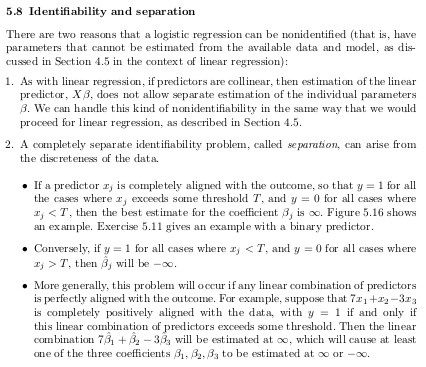
\includegraphics[width=\textwidth,height=0.8\textheight,keepaspectratio=true]{logit_ident}
\end{frame}

\end{document}

